% !TeX root = ../b01.tex

\section{Aufgabe BI-3}

\begin{task}
    Die folgende Graphik zeigt für $n=200$ Beobachtungen eines Merkmals $X$ die empirische Verteilungsfunktion:

    \begin{figure}[H]
        \begin{center}
            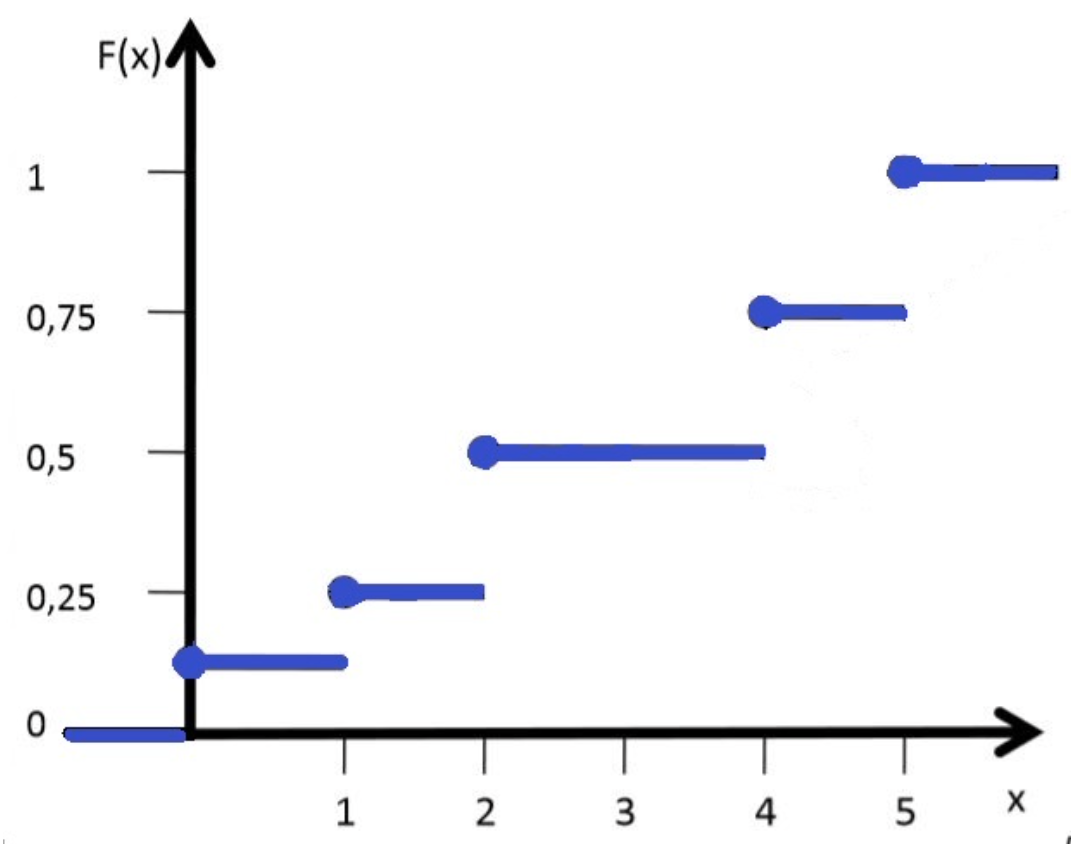
\includegraphics[width=0.3\textwidth]{assets/task3.png}
        \end{center}
    \end{figure}

    \begin{enumerate}
        \item[(a)] Welche Merkmalsausprägungen (verschieden, positiv) wurden für $X$ beobachtet?
    \end{enumerate}
\end{task}

Aus der Graphik lassen sich die folgenden Sprünge ablesen, welche die beobachteten Merkmalsausprägungen von $X$ darstellen: $\lbrace 0, 1, 2, 4, 5 \rbrace$.

\begin{task}
    \begin{enumerate}
        \item[(b)] Bestimmen Sie die absoluten Häufigkeiten der Merkmalsausprägungen von $X$.
    \end{enumerate}
\end{task}

$$
\begin{aligned}
    \forall j\in\lbrace 1,2,\ldots,\ell\rbrace:
    r_j &= \begin{cases}
        F(x_j)              &\text{für}~j=0 \\
        F(x_j) - F(x_{j-1}) &\text{für}~j>0
    \end{cases} \\
    h_j &= n\cdot r_j
\end{aligned}
$$

\begin{table}[H]
\centering
\begin{tabular}{c|clll}
    $j$ & $a_j$ & $F(x_j)$ & $r_j$ & $h_j$ \\ \hline
    1   & $0$   & 0.125    & 0.125 & 25    \\
    2   & $1$   & 0.25     & 0.125 & 25    \\
    3   & $2$   & 0.5      & 0.25  & 50    \\
    4   & $4$   & 0.75     & 0.25  & 50    \\
    5   & $5$   & 1        & 0.25  & 50    \\
\end{tabular}
\end{table}
\nopagebreak
Die absoluten Häufigkeiten $h_j$ können aus der oben dargestellten Tabelle abgelesen werden.

\pagebreak

\begin{task}
    \begin{enumerate}
        \item[(c)] Berechnen Sie das arithmetische Mittel $\overline{x}$ sowie die (korrigierte) Varianz $s^2$ der Daten.
    \end{enumerate}
\end{task}

{\allowdisplaybreaks
    \begin{align*}
        \overline{x} &= \sum_{j=1}^m a_j\cdot r_j \\*
        &= 0\cdot 0.125 + 1\cdot 0.125 + 2\cdot 0.25 + 4\cdot 0.25 + 5\cdot 0.25 \\*
        \Rightarrow \overline{x} &= 2.875 \\
        \nonumber \\
        %
        s^2 &= \frac{1}{n-1} \sum_{j=1}^m (x_j - \overline{x})^2 \\*
        &= \frac{1}{200-1} \big((0 - 2.875)^2 + (1 - 2.875)^2 + (2 - 2.875)^2 \\*
            &\qquad\qquad\quad + (4 - 2.875)^2 + (5 - 2.875)^2 \big) \\*
        &\approx \frac{1}{199} \cdot 18.3281 \\*
        \Rightarrow s^2 &\approx 0.0921
    \end{align*}
}

Insgesamt ergibt sich ein arithmetisches Mittel von $\overline{x} = 2.875$ und eine (korrigierte) Varianz von $s^2 \approx 0.0921$.


\begin{task}
    \begin{enumerate}
        \item[(d)] Es wird eine Stichprobe mit zehn weiteren Beobachtungen erhoben. Alle zehn Beobachtungen haben den Wert $3$. Wie lauten dann die neuen relativen Häufigkeiten der Merkmalsausprägungen von $X$ für die um jene Beobachtungswerte erweiterte Stichprobe?
    \end{enumerate}
\end{task}

neuer Stichprobenumfang $n' = 200+10 = 210$

\begin{table}[H]
\centering
\begin{tabular}{c|cc|c}
    $j'$ & $a'_j$ & $h'_j$ & $r'_j$                  \\ \hline
    1    & $0$    & 25     & $25/210 \approx 0.1190$ \\
    2    & $1$    & 25     & $25/210 \approx 0.1190$ \\
    3    & $2$    & 50     & $50/210 \approx 0.2381$ \\
    4    & $3$    & 10     & $10/210 \approx 0.0476$ \\
    5    & $4$    & 50     & $50/210 \approx 0.2381$ \\
    6    & $5$    & 50     & $50/210 \approx 0.2381$
\end{tabular}
\end{table}

Die neuen relativen Häufigkeiten $r'_j$ lassen sich aus der Tabelle ablesen.
